\documentclass{sig-alternate}
\usepackage[english]{babel}
\usepackage{url}
\usepackage{booktabs}
\usepackage{amsmath}
\usepackage{graphicx}
\usepackage{fancyhdr}
\usepackage{subcaption} 
\setlength{\heavyrulewidth}{1,2pt}
\setlength{\lightrulewidth}{0,7pt}

\cfoot{\thepage}
\pagenumbering{arabic}
\setcounter{page}{265}

\renewcommand{\headrulewidth}{0pt}
\pagestyle{fancy}
\fancyhf{}
\rhead{UMAP 2017 Short Paper}
\lhead{UMAP'17, July 9-12, 2017, Bratislava, Slovakia}


\begin{document}



\title{Interactive Prior Elicitation of Feature Similarities for Small
Sample Size Prediction}

\numberofauthors{3}

\author{
\alignauthor
Homayun Afrabandpey\\
       \affaddr\small\mbox{Helsinki Institute for Information}\\
       \affaddr\small\mbox{Technology HIIT, Dept. of Computer}\\
       \affaddr\small{Science, Aalto University}\\
       \email\small{homayun.afrabandpey@aalto.f}
\alignauthor
Tomi Peltola\\
       \affaddr\small\mbox{Helsinki Institute for Information}\\
       \affaddr\small\mbox{Technology HIIT, Dept. of Computer}\\
       \affaddr\small{Science, Aalto University}\\
       \email\small{tomi.peltola@aalto.fi}
\alignauthor
Samuel Kaski\\
       \affaddr\small\mbox{Helsinki Institute for Information}\\
       \affaddr\small\mbox{Technology HIIT, Dept. of Computer}\\
       \affaddr\small{Science, Aalto University}\\
       \email\small{samuel.kaski@aalto.fi}
}

\maketitle

\begin{abstract}

Regression under the "small n, large p" condition, of small sample size n and large number of features p in the learning data set, is a recurring setting in which learning from data is difficult. With prior knowledge about relationships of the features, p can effectively be reduced, but explicating such prior knowledge is difficult for experts. In this paper we introduce a new method for eliciting expert prior knowledge about the similarity of the roles of features in the prediction task. The key idea is to use an interactive multidimensional-scaling (MDS) type scatterplot display of the features to elicit the similarity relationships, and then use the elicited relationships in the prior distribution of prediction parameters. Specifically, for learning to predict a target variable with Bayesian linear regression, the feature relationships are used to construct a Gaussian prior with a full covariance matrix for the regression coefficients. Evaluation of our method in experiments with simulated and real users on text data confirm that prior elicitation of feature similarities improves prediction accuracy. Furthermore, elicitation with an interactive scatterplot display outperforms straightforward elicitation where the users choose feature pairs from a feature list.

\bigskip
\chapter{CCS CONCEPTS}

\bullet Computing methodologies \rightarrow{} Machine learning; \bullet Human -
centered computing \rightarrow{} Human computer interaction (HCI);

\bigskip
\chapter{KEYWORDS} \\
Interaction; prior elicitation; regression; small n large p; visualization





\end{abstract}

%\category{TODO}{TODO}{TODO}
%\category{TODO}{TODO}{TODO}

%\terms{Design, Experimentation}

%\keywords{TODO, TODO, TODO}


\section{Introduction}
Regression analysis becomes difficult when the sample size is substantially
smaller than the number of features. "Small n, large p"
refers to the generic class of such problems which arise in different
fields of applied statistics such as personalized medicine \cite{2569992285,I28oKV} and
text data analysis \cite{Forman:2003:EES:944919.944974,Qu:2010:BMR:1873781.1873884}. The problem poses several challenges
to standard statistical methods \cite{Johnstone558612} and demands new concepts
and models to cope with the challenges. An important challenge is

\hrule

{\scriptsize Permission to make digital or hard copies of all or part of this work for personal or
classroom use is granted without fee provided that copies are not made or distributed
for profit or commercial advantage and that copies bear this notice and the full citation
on the first page. Copyrights for components of this work owned by others than ACM
must be honored. Abstracting with credit is permitted. To copy otherwise, or republish,
to post on servers or to redistribute to lists, requires prior specific permission and/or a
fee. Request permissions from permissions@acm.org.
UMAP'17, July 9–12, 2017, Bratislava, Slovakia
\textcopyright 2017 ACM. 978-1-4503-4635-1/17/07. . . $15.00
$DOI: http://dx.doi.org/10.1145/3079628.3079698}


\normalsize that prediction by fitting regression models using traditional techniques
is an ill-posed task in "small n, large p" and is unlikely to be
accurate and reliable. Regularization methods \cite{Tibshirani94regressionshrinkage,Zou98894} have been
proposed to cope with this challenge; however, the improvement
they can give is limited. Additionally, modelling could use prior
information, i.e. information available about the problem prior to
observing the learning data. Prior information is often available
only as the experience and knowledge of experts. Prior elicitation
is the process of quantifying and extracting user's prior knowledge.
The extracted knowledge can be used to improve an underlying
model. The two main questions in the process are how to quantify
the prior knowledge, and how to plug-in the extracted prior
knowledge to the model.
Garthwaite et al. \cite{Garthwaite12} proposed a method of defining the full
prior distribution for a generalized linear model by quantifying
experts' opinions on different statistics such as the median, lower
and upper quantiles. Interactive Principal Component Analysis
(iPCA) \cite{Jeong:2009:IIS:2421899.2421907} supports data analysis of multivariate data sets through
modification of the model parameters by the user. The drawback
of these types of prior elicitation is that they assume users are
experts in the underlying model and not just domain-experts. To
solve this problem, observation-level interaction has been proposed
where the focus is on interaction between the user and the data
rather than model parameters \cite{Liu:2012:DLD:2478276.2478281,DBLP:conf/ieeevast/EndertHMHLN11}. Using the extracted knowledge
from the interaction, the parameters of the underlying model are
tuned to reflect the user's knowledge. In recent work, Daee et al. \cite{Daee65754}
proposed a method of eliciting user's knowledge on the relevance
and/or weight values of single features to improve the predictions
in a sparse linear regression problem. Similarly, Micallef et al. \cite{Micallef:2017:IEK:3025171.3025181}
proposed an interactive visualization to extract user's knowledge
on the relevance of individual features for a prediction task.
In this paper, we present a novel approach on interactive prior
elicitation of pairwise similarities of features in "small n, large p"
prediction task. The proposed approach uses an interactive MDStype
scatterplot of the features to let users give feedback on their
pairwise similarities, in the sense of how similarly they would
affect the predictions. Based on this input, the system learns a
new similarity metric for the features and redraws the scatterplot.
Finally, the learned metric is used to define a prior distribution for
the prediction parameters. The proposed approach shields users
from the technicalities of the underlying model. The contributions
of this paper can be summarized as:

\begin{itemize}
   
    \item User's prior knowledge is quantified as the prior covariance
of the regression coefficients in a Bayesian linear regression
model. Using this interpretation, our system lets the user
manipulate the prior distribution of the model parameter indirectly by his feedback, without having to understand modelling details.

    \item  Feedback is collected on pairwise similarities of the features
rather than the data, parameters or single features.
This type of feedback is complementary to all earlier approaches.

    \item The prior is elicited with an MDS-type of interactive visualization
that has earlier been used for visualizing similarities
of data items

\end{itemize}

Our simulation results and preliminary user study demonstrate that
when collecting pairwise similarity knowledge using the proposed
interactive intelligent interface, users are able to provide more
informative feedback, and the performance of the underlying model
increases in prediction tasks.

\section{Overview}

To motivate our algorithm and for the purpose of clarity, we illustrate
our basic idea with a simple use case. We used the sentiment
data set \cite{P07-1056} which contains text reviews and the corresponding
rating values (taken from www.amazon.com) of four product categories.
Each review is represented using a vector of keywords that
appear in at least 100 reviews within the same category. We focus
on the kitchen appliances category where there are 5149 reviews,
each represented by a feature vector of size 824 \cite{Hernandez-Lobato:2015:EPL:2783156.2783164}. The task is
to learn a model that linearly relates the keywords (which here
are features) to the ratings (outputs) to predict the ratings from
the textual content of the reviews. This is a supervised learning
task where we have a training set of inputs x $\in$ R$^{5149\times824}$ and
outputs y$\in$ R$^{5149\times1}$. To simulate the"small n, large p" paradigm,
we randomly select 100 reviews and their corresponding ratings as
the training set.
A linear regression model for this task can be defined using a
parameter vector $\beta$ = ($\beta$ 1,$\beta$ 2, ..., $\beta$ 824)$\in$ R$^{824\times1}$ . Mathematically, the model is \\ 

{\centering {y=X$\beta$ + $\epsilon$ } \flushright{ (1) }}



where $\in$ $\backsim$ N (0, $\sigma ^{2}_{noise}$I)
is the residual noise. Equation 1 induces
a Gaussian likelihood as y $\mid$ $\beta ,\sigma ^{2}_{noise}$ $\sim$ N (X $\beta$ , $\sigma$ $^{2}_{noise}$ I). The goal is
to learn the posterior distribution of $\beta$  given the training data.
Inferring the posterior of the parameters in the Bayesian setting
requires a prior distribution. In data sets with large sample sizes,
the choice of the prior distribution will have a minor effect on
the posterior inferences; however, since we assumed a "small n,
large p" data set, the role of the prior distribution becomes more
important. Setting prior distributions is a difficult task and requires
knowledge on both the domain and the model parameters. In this
paper, we introduce a method for helping in this task, by learning
and refining a good prior distribution for the prediction parameters
using feedback given by a user. User's knowledge is assumed to be
about the pairwise similarities of the keywords with regard to the
role they have in the prediction task. In other words, we mean that
keywords have a similar effect on the rating values (the values of the
regression coefficients are similar). As an example, keywords "good"
and "excellent" have a similar role in the prediction since both of
them convey information that the user will give a high rating to
the product, while keywords "bad" and "good" are dissimilar.


\begin{figure}[h]
    \centering
    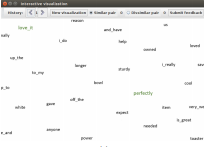
\includegraphics{images/OBRA.png}
    
    \label{obrazoka}
\end{figure}

\begin{figure}[h]
    \centering
    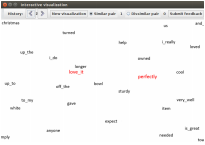
\includegraphics{images/OBRB.png}
    
    \label{obrazokb}
    \caption{\textbf{The scatterplot (a) before submitting feedback, and
(b) after submitting feedback and requesting a new visualization.
The scatterplots are zoomed in suitably to better show
the keywords}}
\end{figure}


our system. Keywords (features) are visualized to the user on the
scatter plot, where she can zoom in/out by scrolling down/up the
mouse. The user investigates the distances among keywords and
decides whether two keywords should be closer to each other (similar)
or farther away from each other (dissimilar) based on her prior
knowledge. As an example, the user concluded that according to her
prior knowledge, the distances between keywords \textbf{"love it"} and
\textbf{"perfectly"} should be less than what is shown in the scatterplot.
She selects these keywords by clicking on them (their color will
change to green as shown in Figure 1a), selecting similar/dissimilar
box in the menu bar and clicking on the submit button. Then the
user can ask for a new visualization (\textbf{New Visualization} button in
Figure 1) to see the effect of her feedback on the distances between
keywords (Figure 1b), or she can continue giving more feedback
according to current distances. As shown in Figure 1b, the one feedback
given by the user modifies the distances between keywords,
however it was not informative enough to make distances perfect.
This will iterate until the user is satisfied with the visualization.
The knowledge extracted from the user is used to build a proper
covariance matrix for the prior distribution of the prediction parameter
$\beta$ . Finally, using the obtained prior, we compute the posterior
of the prediction parameters.


\section{INTERACTIVE PRIOR ELICITATION OF PAIRWISE SIMILARITIES}

We reformulate the Interactive Neighbor Retrieval Visualizer \cite{PE.EuroVisShort.EuroVisShort2013.049-053} to
a method for prior elicitation on features. To visualize the features 
for the user, we use the original data space as the representation
for the features in the high-dimensional space. More precisely, we
define $\int_i=[x_{li}, ... ,x_{ni}]^T$ as the original representation
of the $i^{th}$ element of the
$n^{th}$ sample. With this definition, we have D features, each of which
is an n-dimensional
vector. We define \{$g_i$\}$^D_{i=1}$ as the corresponding low-dimensional
projections of \{$\int_i$\}$^D_{i=1}$,to be learned from user feedback.
At each iteration t, we define the similarity matrix of the features
in the high-dimensional space as 
$P^t=\left[P^t_{j\mid i}\frac{exp(-\mid \mid \int_{i}-\int_{j}\mid \mid_{A^t}^{t} \diagup\sigma^2_i)       }{\sum_{k\neq i }exp(-\mid \mid \int_{i}-\int_{j}\mid \mid_{A^t}^{t} \diagup\sigma^2_i)  }\right]^D_{i,j=1}$,
where $A^t$is the unknown similarity metric between the features,
$\mid\mid\int_{i} -\int_{j}\mid \mid^2_A=(\int_{i} -\int_{j})^TA(\int_{i} -\int_{j}) $
and 
$\sigma^2_i$
is a scaling parameter.
The unknown similarity metric
$A^t$
encodes the user feedback and
is learned iteratively by interaction with the user. The metric is
initialized to unit matrix.
To find the location of the points in the visualization space at
iteration t, an analogous matrix is defined for the low-dimensional
projections:
$\varrho^t=\left[q^t_{j\mid i}=\frac{exp(-\mid\mid g^t_i - g^t_j\mid\mid ^2\diagup\sigma^2_i)}{\sum_{k\neq i} exp(-\mid\mid g^t_i - g^t_k\mid\mid ^2\diagup\sigma^2_i} \right]^D_{i,j=1}$.
Finally, the locations of the points in the low-dimensional space are
obtained by optimizing the following expected cost function \cite{PE.EuroVisShort.EuroVisShort2013.049-053}:
$E[C]=E_{A\mid F}[\lambda E_i [KL(P_i,Q_i)]+(1-\lambda )E_i [KL(Q_i,P_i)]]$
where $E_{A\mid F}$ denotes the expectation over the posterior distribution
of the learned metric given the feedbacks F , and $E_i$ is expectation
over the training set points. Since the high-dimensional distributions $P_i$ 
are functions of the unknown metric A, the cost function
is represented as the expectation over the possible metrics. The
parameter $\lambda \in $ [0.1] controls the relative importance of recall and
precision of the display \cite{Venna:2010:IRP:1756006.1756019}. The final similarity metric $A^{final}$,
learned in the last iteration of user interaction, is used to define a
prior distribution for the regression weights according to equations
5 and 6:
$C=\left[c_{i,j}=exp(-\frac{\mid\mid f_i-f_j\mid\mid^2_{A^{final}}}{2\sigma^2}) \right]^D_{i,j=1}$, \hfill{(5)}
$\beta\sim\it{N}(0,\sigma^2_{noise}\tau^2C)$,\hfill{(6)}
where $\sigma$ and $\tau$ are scalar scale parameters. In our implementation,
the value of $\sigma$ is set by cross-validation.
By defining this prior distribution for the regression coefficients,
and gamma prior distributions on $\tau^{-2}$ and $\sigma^{-2}_{noise}$,
 the posterior distribution is analytically intractable, but can be efficiently approximated
using Variational Bayes (e.g., \cite{Bishop:2006:PRM:1162264}[Chapter 10]). This
gives a Gaussian posterior approximation for $\beta$.Pseudocode of the
proposed method is presented in Algorithm 1.
\\
\section{SIMULATION EXPERIMENT}

We conducted a simulated study on the data set introduced in
Section 2 with two scenarios where a simulated user (i) gives all
feedbacks at once, and (ii) gives feedback sequentially. As baselines,
we used Bayesian linear regression with unit prior covariance and

\hrule{}
Algorithm 1: Interactive Prior Elicitation Pseudocode
\hrule{}

\begin{enumerate}
    \item Set $A^0$ = I and t = 0
    \item \textbf{while} user gives more feedback \textbf{do}
        \begin{description}
            \item [b.] Optimize the cost function 4 using the metric $A^t$ and find
the position of the features in the low-dimensional space, $[g^t_i]^D_{i=1}$, at iteration t.
            \item [c.] Ask the user to give feedback about the similarity of the
role of the features.
            \item [d.] Set t = t + 1.
            \item [e.] Learn the new metric $A^t$ using the method introduced in
\cite{Yang:2007:BAD:3020488.3020542} and the user feedback.
        \end{description}
        \item Compute the matrix \textbf{C} using $A^{final}$ (Eq. 5) and define a prior
distribution for the weights as $\beta\sim\it{N}(0,\sigma^2_{noise}\tau^2C)$.
        \item Compute the posterior of the weights and use that to predict
output for a new sample.
\end{enumerate}

\hrule{}

Bayesian linear regression with the prior covariance used in the
first round of our method ("Without Feedback" in the following,
since the prior is obtained by setting \textbf{A = I} and without using feedback).
We used a set of 3149 randomly selected reviews with their
corresponding ratings to construct the simulated user. This is done
by using the mean of the posterior distribution of the regression
coefficient vector of a Bayesian linear regression model trained
on the randomly selected data. The simulated user assumes two
similarity clusters: (i) features with the highest 30 regression coefficients
and (ii) features with the lowest 30 regression coefficients.
Features in these two clusters are dissimilar to each other. Since
there are enough samples (3149) compared to the dimensionality
of the data (824), the posterior mean of the regression coefficient
is a good representative of the true values of the feature weights
and consequently the similarity of the role of the features in the
prediction task.
The remaining samples are randomly partitioned into training
and test sets. The results reported in this section are averaged over
10 simulated user construction iterations and 50 random training
data selection. Figure 2a shows simulation results for the first scenario,
in which the proposed method is evaluated with an increasing
number of randomly selected training samples, from 50 to 500. Figure
2b shows the changes of Mean Squared Errors (MSE) on the
test data with 100 randomly selected training samples when the
simulated user gives feedback sequentially in 60 rounds; round 0
works without feedback. The simulated user gives 10 similarity
feedback and 10 dissimilarity feedback in each round.
From Figure 2, it can be concluded that assuming pairwise similarity/dissimilarity
knowledge from the user, the proposed method
improves the predictions by extracting prior knowledge.

\section{USER STUDY}

We conducted a user study on 10 university students to empirically
evaluate our two hypotheses that (i) collecting prior knowledge on
the pairwise similarity of the features improves predictions, and
(ii) the interactive interface helps users to give better feedback and
consequently improves the predictions more. To evaluate the first
hypothesis, we consider the same baselines used in the previous
section. To evaluate the second hypothesis, we implemented two
versions of our system, both with the same underlying model, but

\begin{figure}[h!]
  \centering
  \begin{subfigure}[b]{0.4\linewidth}
    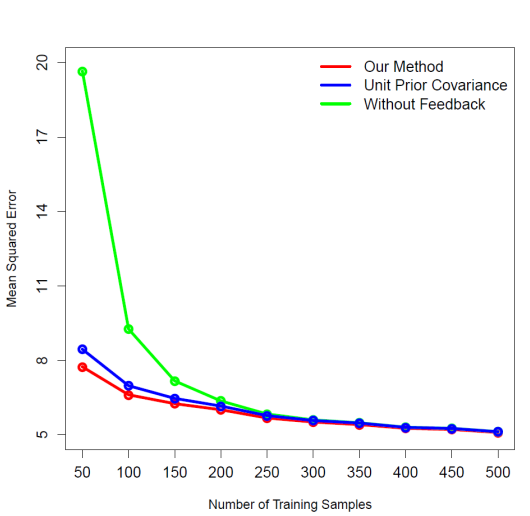
\includegraphics[width=\linewidth]{images/OBRAZOK_GRAF_A.png}
   \caption{}
  \end{subfigure}
  \begin{subfigure}[b]{0.4\linewidth}
    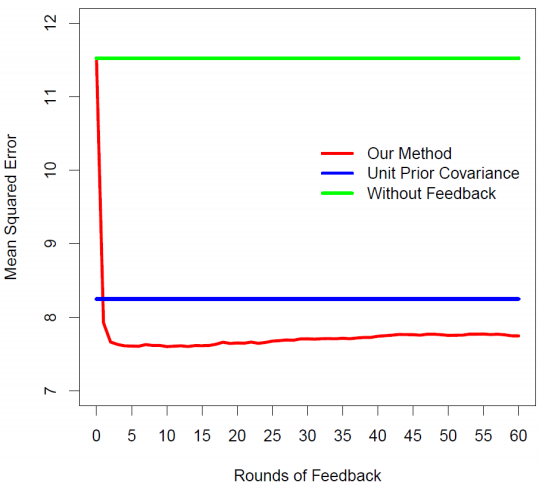
\includegraphics[width=\linewidth]{images/OBRAZOK_GRAF_B.png}
   \caption{}
  \end{subfigure}
 \caption{\textbf{ Simulation results for (a) batch feedback, (b) sequential
feedback.}}
  \label{obrazokgraf}
\end{figure}

with different interfaces: the proposed interactive interface and a
simple non-interactive list visualization of the features. In the list
visualization, the order of the features is random and fixed during
the whole experiment for a user. The user goes through the list and
selects the pairs which are similar or dissimilar according to her
prior knowledge and gives feedback on them. As far as we know,
there are no earlier methods for the same task.
We designed a between-subject study, where each participant
performed two prior elicitation tasks with different interfaces and
different data collections: the sentiment data set introduced in Section
2 and the reviews from the Yelp data set challenge (www.yelp.
com/dataset\_challenge). Users were asked to give feedback on pairwise
similarity/dissimilarity of the words in the role they have in
the prediction. For the Yelp data, we used a subset with 4086 reviews.
In both data sets, we set a threshold on the tf-idf values (see \cite{Jones72astatistical}
) of the words to choose 300 words. To simulate a "small n, large
p" training data, we randomly selected five subsets of each data set
with 100 samples, and used the rests for test. Therefore, the training
set for each task contains 100 samples and 300 features. Each of
the selected five subsets (from each data set) was used once for the
interactive interface and once for the non-interactive interface with
different users. Users interact with each interface for 20 rounds and
give 5 feedbacks (similarity/dissimilarity) per round. The study was
balanced with respect to the combination of the type of interface,
task and order. After both tasks, a short semi-structured interview
was conducted with each participant.
Figures 3a and 3b show MSEs on test data as a function of the
number of feedback iterations for the two data sets. According to
the figures, extracted prior knowledge improves the mean squared
errors of the predictions compared to both baselines. The difference
between the MSE values obtained by the interactive interface and
the non-interactive interface shows the amount of improvement
made to the predictions using the interface. To test the statistical
significance of the improvements, we used the procedure introduced
in \cite{Micallef:2017:IEK:3025171.3025181}. The distance between the average curves in the last round
(round 20 in Figure 3) is used as the test statistics. By assuming that
there is no difference between the results obtained by the interactive
interface and other methods, we compute the distribution of the test
statistics by performing $10^5$ permutations of the labels (interactive
interface, non-interactive interface, etc.). Finally, the proportion
of the permutations with higher values of test statistics compared
to the test statistics using true labels, is used as p-value of the
significance test. Based on this test, the improvements made by our
interactive interface against the "Unit Prior Covariance" (p = 0.048
for the sentiment and p = 0.016 for the YELP data set) and the
"Without Feedback" (p = 0.0 for the sentiment and p = 0.0 for the
YELP data set)  baselines in both data sets are statistically significant, while for against the non-interactive interface, the improvements
are not statistically significant (p = 0.73 for the sentiment and
p = 0.56 for the YELP data set) which might be due to the small
number of users.
It should be noted that since only a small portion of the words
are meaningfully related to the rate prediction task, i.e. most of
the words are verbs (am, is, etc.) or subjects (I, he, etc.) which are
difficult for the user to give feedback, users gave their best feedback
in the first couple of rounds which causes prior elicitation to best
improve the prediction errors in the first half of the rounds. But, in
the second half, prediction errors either improve slowly because
of the repetitive feedbacks given by the user, or even sometimes
drop since some users gave feedback on irrelevant words. In the

\begin{figure}[h!]
  \centering
  \begin{subfigure}[b]{0.4\linewidth}
    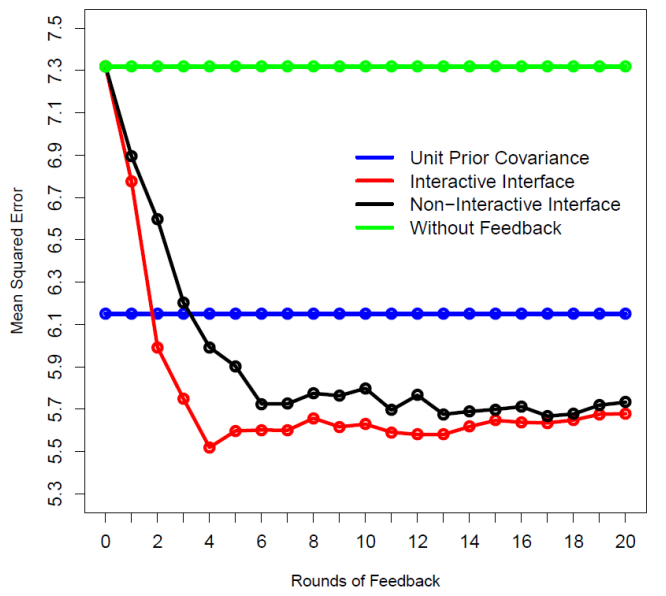
\includegraphics[width=\linewidth]{images/OBRAZOKGRAF2A.png}
   \caption{}
  \end{subfigure}
  \begin{subfigure}[b]{0.4\linewidth}
    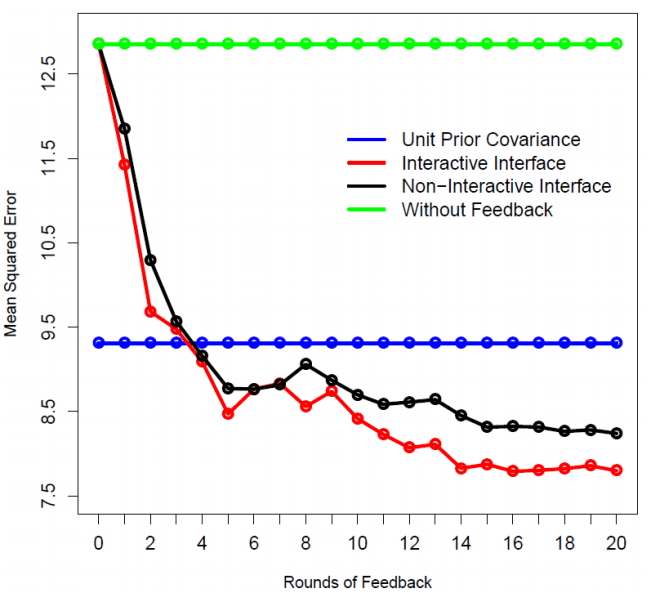
\includegraphics[width=\linewidth]{images/OBRAZOKGRAF2B.png}
   \caption{}
  \end{subfigure}
\caption{ \textbf{ Changes of prediction MSE by increasing number
of feedbacks for (a) the subset of the sentiment data set and
(b) the subset of the Yelp data set.}}
  \label{obrazokgraf}
\end{figure}

interview, 8 out of 10 users reported that the intelligent interface
helped them to accomplish the task. However, 5 users stated that
they preferred the simple interface over the intelligent one. This
is not surprising since people often prefer simpler systems over
more complex ones \cite{Hearst:2009:SUI:1631268} even if the complex system benefits them
in accomplishing the required task.

\section{DISCUSSION AND CONCLUSION}

In this paper, we presented a new method and a prototype implementation
of an interactive prior elicitation system which elicits
an expert's prior knowledge on feature similarities to improve prediction
accuracy. The system involves an intelligent user interface
which helps the user in the interaction. We believe that this is an
important step toward more efficient interactive prior elicitation
methods. The main novelties are the type of feedback assumed from
the user and the interpretation of the extracted knowledge as prior
covariance for the parameter of the linear regression model.
In the current implementation, we pruned the number of features
to avoid overwhelming the user; however, for the general case of
a large number of features, we are working on an active learning
version of the method to prioritize the feature pairs and allow
scaling up to a much larger number of features.

\section{ACKNOWLEDGMENTS}

This work has been supported by the Academy of Finland (Finnish
Center of Excellence in Computational Inference Research COIN;
grants 294238 and 292334). We acknowledge the computational
resources provided by the Aalto Science-IT project.



\bibliographystyle{abbrv}
\bibliography{Zdroje}

\balancecolumns

\end{document}
